\documentclass[12pt,a4paper]{article}
\usepackage[utf8]{vietnam}
\usepackage{amsmath,amssymb}
\usepackage{tabularx}
\usepackage{tikz}
\usetikzlibrary{calc,angles,quotes,arrows.meta,patterns}
\usepackage{xcolor}
\usepackage{enumitem}
\usepackage{fancyhdr}
\usepackage[top=1.2cm, bottom=1.2cm, left=1.5cm, right=1.5cm]{geometry}
\usepackage[dethi]{ex_test}
\SAOPTN{widthSA=2.6,heightSA=0.62}

\setlength{\headheight}{15pt}
\setlength{\parskip}{0pt}

% Dòng kẻ chấm mờ chuẩn viết tay
\newcommand{\dongke}[1]{%
  \begingroup%
  \setlength{\parskip}{0pt}%
  \baselineskip=18.5pt%
  \vspace{1.0mm}%
  \foreach \i in {1,...,#1}{%
    \noindent{\color{gray!60}\dotfill}\par%
  }%
  \vspace{0.6mm}%
  \endgroup%
}

\pagestyle{fancy}
\fancyhf{}
\rhead{\textit{Môn Toán 6 -- Đề số 3}}
\lhead{\textit{Bộ đề ôn tập Giữa học kì I}}
\cfoot{\thepage}

\begin{document}

% --- KHUNG TIÊU ĐỀ ĐỀ THI ---
\noindent
\begin{tabularx}{\linewidth}{X r}
\textbf{TRƯỜNG THCS: \dotfill} & \textbf{ĐỀ KIỂM TRA ĐỊNH KỲ GIỮA HỌC KỲ I} \\
\textbf{Họ và tên: \dotfill} & \textbf{NĂM HỌC 2026 -- 2027} \\
\textbf{Lớp: \dotfill \quad SBD: \dotfill} & \textbf{Môn: TOÁN 6} \\
\hline
\end{tabularx}
\vspace{2mm}

\begin{center}
  \textbf{\large ĐỀ ÔN TẬP GIỮA HỌC KỲ I -- ĐỀ SỐ 3}\\
  \textit{Thời gian làm bài: 90 phút (Không kể thời gian phát đề)}
\end{center}
\vspace{1mm}

% --- PHẦN I ---
\noindent\textbf{\large PHẦN I. CÂU TRẮC NGHIỆM NHIỀU PHƯƠNG ÁN LỰA CHỌN (3,0 điểm)}

\textit{Thí sinh trả lời từ câu 1 đến câu 12. Mỗi câu hỏi thí sinh chỉ chọn một phương án duy nhất.}

\vspace{1mm}
\begin{ex}
Cho tập hợp $A = \{1; 2; a; b\}$. Khẳng định nào dưới đây là sai?
\choice
{$1 \in A$}
{$a \in A$}
{$5 \notin A$}
{\True $b \notin A$}
\end{ex}

\begin{ex}
Tập hợp nào dưới đây là tập hợp số tự nhiên?
\choice
{$\mathbb{N} = \{1; 2; 3; \dots\}$}
{$\mathbb{N} = \{0; 1; 2; 3; \dots; 100\}$}
{\True $\mathbb{N} = \{0; 1; 2; 3; \dots\}$}
{$\mathbb{N} = \{0; 2; 4; 6; \dots\}$}
\end{ex}

\begin{ex}
Số nào sau đây là bội của $17$?
\choice
{\True $51$}
{$54$}
{$56$}
{$63$}
\end{ex}

\begin{ex}
Một nhà kho có $240$ bao gạo, chia đều vào $8$ dãy kệ. Sau đó, người ta lấy ra $15$ bao ở mỗi dãy kệ để chuyển đi nơi khác. Hỏi nhà kho còn lại bao nhiêu bao gạo?
\choice
{$105$ bao}
{$115$ bao}
{\True $120$ bao}
{$135$ bao}
\end{ex}

\begin{ex}
Công thức tính chu vi của hình vuông có độ dài cạnh $a$ là:
\choice
{$C = a$}
{\True $C = 4a$}
{$C = 3a$}
{$C = 5a$}
\end{ex}

\begin{ex}
Trong các hình dưới đây, hình nào là hình thoi?\begin{center}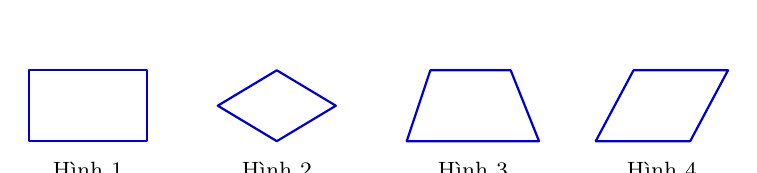
\begin{tikzpicture}[scale=0.6, line cap=round, line join=round]\begin{scope}[xshift=0cm]\draw[thick, blue!80!black] (0,0) rectangle (2.5,1.5);\node[below=4pt, font=\footnotesize] at (1.25,0) {Hình 1};\end{scope}\begin{scope}[xshift=4cm]\draw[thick, blue!80!black] (1.25,1.5) -- (2.5,0.75) -- (1.25,0) -- (0,0.75) -- cycle;\node[below=4pt, font=\footnotesize] at (1.25,0) {Hình 2};\end{scope}\begin{scope}[xshift=8cm]\draw[thick, blue!80!black] (0.5,1.5) -- (2.2,1.5) -- (2.8,0) -- (0,0) -- cycle;\node[below=4pt, font=\footnotesize] at (1.4,0) {Hình 3};\end{scope}\begin{scope}[xshift=12cm]\draw[thick, blue!80!black] (0.8,1.5) -- (2.8,1.5) -- (2,0) -- (0,0) -- cycle;\node[below=4pt, font=\footnotesize] at (1.4,0) {Hình 4};\end{scope}\end{tikzpicture}\end{center}
\choice
{Hình 1}
{\True Hình 2}
{Hình 3}
{Hình 4}
\end{ex}

\begin{ex}
Đọc lũy thừa $6^3$ và nêu cơ số, số mũ của nó:
\choice
{\True Sáu mũ ba; cơ số là $6$, số mũ là $3$}
{Sáu mũ ba; cơ số là $3$, số mũ là $6$}
{Ba mũ sáu; cơ số là $3$, số mũ là $6$}
{Ba mũ sáu; cơ số là $6$, số mũ là $3$}
\end{ex}

\begin{ex}
Khi viết gọn tích $3 \cdot 2 \cdot 6^2 \cdot 6$ dưới dạng một lũy thừa, kết quả đúng là:
\choice
{$3^3 \cdot 2^2$}
{$6^3$}
{\True $6^4$}
{$2^3 \cdot 3^2$}
\end{ex}

\begin{ex}
Khẳng định nào sau đây là đặc trưng về cạnh của hình vuông?
\choice
{Hai cạnh đối bằng nhau}
{Hai đường chéo bằng nhau}
{\True Bốn cạnh bằng nhau}
{Hai đường chéo vuông góc}
\end{ex}

\begin{ex}
Cho hình thang có độ dài hai đáy lần lượt là $6\text{ cm}$ và $10\text{ cm}$, chiều cao là $5\text{ cm}$. Diện tích của hình thang đó là:
\choice
{\True $40\text{ cm}^2$}
{$50\text{ cm}^2$}
{$60\text{ cm}^2$}
{$70\text{ cm}^2$}
\end{ex}

\begin{ex}
Cho tam giác đều $MNP$ có cạnh $MP = 6\text{ cm}$. Độ dài các cạnh $MN$ và $NP$ lần lượt là:
\choice
{$2\text{ cm}; 4\text{ cm}$}
{$3\text{ cm}; 3\text{ cm}$}
{$1\text{ cm}; 5\text{ cm}$}
{\True $6\text{ cm}; 6\text{ cm}$}
\end{ex}

\begin{ex}
Một hình thoi có độ dài hai đường chéo lần lượt là $2\text{ cm}$ và $4\text{ cm}$. Diện tích của hình thoi đó là:
\choice
{\True $4\text{ cm}^2$}
{$6\text{ cm}^2$}
{$8\text{ cm}^2$}
{$2\text{ cm}^2$}
\end{ex}


\vspace{1mm}
\noindent\textbf{BẢNG TRẢ LỜI TRẮC NGHIỆM PHẦN I:}
\begin{center}
\begin{tabular}{|c|c|c|c|c|c|c|c|c|c|c|c|c|}
\hline
\textbf{Câu} & \textbf{1} & \textbf{2} & \textbf{3} & \textbf{4} & \textbf{5} & \textbf{6} & \textbf{7} & \textbf{8} & \textbf{9} & \textbf{10} & \textbf{11} & \textbf{12} \\
\hline
\textbf{Chọn} & \rule{0pt}{0.65cm} & & & & & & & & & & & \\
\hline
\end{tabular}
\end{center}
\vspace{2mm}

\setcounter{ex}{0}
\noindent\textbf{\large PHẦN II. CÂU TRẮC NGHIỆM ĐÚNG SAI (2,0 điểm)}

\textit{Thí sinh trả lời câu 1 và câu 2. Trong mỗi ý a), b), c), d) ở mỗi câu, thí sinh chọn đúng hoặc sai.}

\vspace{1mm}
\begin{ex}
Cho hình vuông $MNPQ$ có cạnh bằng $4\text{ cm}$. Các khẳng định sau đây đúng hay sai?
\choiceTF
{\True $MN = NP = PQ = QM = 4\text{ cm}$}
{$MN$ và $NQ$ song song với nhau}
{Mỗi góc ở các đỉnh của hình vuông bằng nhau và bằng $60^\circ$}
{\True Dùng thước và ê-ke vẽ được hình vuông $MNPQ$ có cạnh bằng $4\text{ cm}$}
\end{ex}

\begin{ex}
Cho các số: $355, 360, 257, 1617, 152$. Các khẳng định sau đây đúng hay sai?
\choiceTF
{\True Số $360$ chia hết cho $9$}
{Số $1617$ chia hết cho $9$}
{Trong các số đã cho, có đúng hai số chia hết cho $9$}
{\True Số $257$ và số $152$ đều không chia hết cho $9$}
\end{ex}


\noindent\textbf{BẢNG TRẢ LỜI PHẦN II:}
\begin{center}
\begin{tabular}{|c|c|c|c|c||c|c|c|c|c|}
\hline
\textbf{Câu 1} & \textbf{a)} & \textbf{b)} & \textbf{c)} & \textbf{d)} & \textbf{Câu 2} & \textbf{a)} & \textbf{b)} & \textbf{c)} & \textbf{d)} \\
\hline
\textbf{Đ/S} & \rule{0pt}{0.6cm} & & & & \textbf{Đ/S} & & & & \\
\hline
\end{tabular}
\end{center}
\vspace{2mm}

\setcounter{ex}{0}
\noindent\textbf{\large PHẦN III. CÂU HỎI TRẢ LỜI NGẮN (2,0 điểm)}

\textit{Thí sinh trả lời câu 1 và câu 2. Điền kết quả số vào ô trống tương ứng.}

\vspace{1mm}
\begin{ex}
Số lượng các số nguyên tố nhỏ hơn $10$ là bao nhiêu? \shortans{$4$}
\end{ex}

\begin{ex}
Có bao nhiêu số tự nhiên $n$ thỏa mãn $1 < n \le 9$? \shortans{$8$}
\end{ex}


\setcounter{ex}{0}
\noindent\textbf{\large PHẦN IV. TỰ LUẬN (3,0 điểm)}

\textit{Thí sinh trình bày chi tiết lời giải vào giấy làm bài.}

\vspace{1mm}
\begin{ex} (1.0 điểm)
Thực hiện phép tính:
\begin{enumerate}[label=\textbf{\alph*)}, leftmargin=0.8cm, itemsep=2pt]
\item $475 + 170 + 325 + 330$
\item $89 \cdot 54 + 45 \cdot 89 + 89$
\item $120 : \left\{ 54 - \left[ 50 : 2 - (3^2 - 2 \cdot 4) \right] \right\}$
\end{enumerate}
\end{ex}
\vspace{1.5mm}

\begin{ex} (0.75 điểm)
Tìm số tự nhiên $x$, biết:
\begin{enumerate}[label=\textbf{\alph*)}, leftmargin=0.8cm, itemsep=2pt]
\item $x - 15 = 2025$
\item $39 + (x - 47) = 160$
\end{enumerate}
\end{ex}
\vspace{1.5mm}

\begin{ex} (0.75 điểm)
Mảnh vườn nhà ông An có dạng như hình vẽ dưới đây:\
\begin{center}
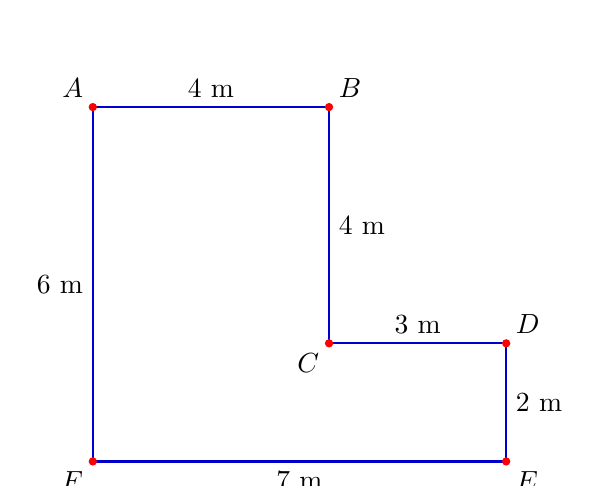
\begin{tikzpicture}[scale=0.75, line cap=round, line join=round]
  \coordinate (F) at (0,0); \coordinate (E) at (7,0); \coordinate (D) at (7,2);
  \coordinate (C) at (4,2); \coordinate (B) at (4,6); \coordinate (A) at (0,6);
  \draw[thick, blue!80!black] (F) -- (E) -- (D) -- (C) -- (B) -- (A) -- cycle;
  \foreach \p in {A,B,C,D,E,F} \fill[red] (\p) circle (2pt);
  \node[above left] at (A) {$A$};
  \node[above right] at (B) {$B$};
  \node[below left] at (C) {$C$};
  \node[above right] at (D) {$D$};
  \node[below right] at (E) {$E$};
  \node[below left] at (F) {$F$};
  \node[above] at (2,6) {$4\text{ m}$};
  \node[right] at (4,4) {$4\text{ m}$};
  \node[above] at (5.5,2) {$3\text{ m}$};
  \node[right] at (7,1) {$2\text{ m}$};
  \node[below] at (3.5,0) {$7\text{ m}$};
  \node[left] at (0,3) {$6\text{ m}$};
\end{tikzpicture}
\end{center}
\begin{enumerate}[label=\textbf{\alph*)}, leftmargin=0.8cm, itemsep=2pt]
\item Ông An rào xung quanh mảnh vườn bằng dây thép gai. Hỏi ông An mua hết bao nhiêu tiền dây thép gai, biết mỗi mét dây thép gai có giá $50\,000$ đồng?
\item Tính diện tích mảnh vườn của ông An.
\end{enumerate}
\end{ex}
\vspace{1.5mm}

\begin{ex} (0.5 điểm)
Cho tổng $B = 5 + 5^2 + 5^3 + \dots + 5^8$. Chứng minh rằng $B$ chia hết cho $30$.
\begin{enumerate}[label=\textbf{\alph*)}, leftmargin=0.8cm, itemsep=2pt]
\item Chứng minh $B \ \vdots \ 30$.
\end{enumerate}
\end{ex}
\vspace{1.5mm}


\begin{center}
\rule{4cm}{0.4pt}\\
\textit{--- HẾT ---}
\end{center}
\end{document}
